\documentclass[11pt]{article}
\usepackage[margin=1in]{geometry}
\usepackage{amsmath,amssymb}
\usepackage{graphicx}
\usepackage[hidelinks]{hyperref}

\newcommand{\Lip}{\operatorname{Lip}}
\newcommand{\TP}{\operatorname{TP}}
\newcommand{\TC}{\operatorname{TC}}
\newcommand{\KR}{\operatorname{KR}}
\newcommand{\F}{\mathcal F}
\newcommand{\M}{\mathcal M}

\title{Literature Already Answered: Set-Theoretic Dichotomy for TC/KR Density}
\author{Automatic Math Discovery Run \texttt{fa\_banach\_001}}
\date{June 19, 2026}

\begin{document}
\maketitle

\section*{Status}

This is a \textbf{literature-already-answered packet} for Remark 1.14 of Ostrovska and
Ostrovskii, \emph{Generalized transportation cost spaces}, arXiv:1902.10334
\cite{OO2019}. Raad's characterization gives the exact criterion needed for
the source question. The supporting paper does not appear to cite this source
remark directly, so the identification below records the bridge: the completion
of \(\TP(M)\) is the Lipschitz-free space \(\F(M)\).

\section*{Source Question}

The source paper proves Theorem 1.13: if \(M\) is Polish, then
\((\TP(M),\|\cdot\|_{\TC})\) is dense in the
Kantorovich--Rubinstein measure space \((\M,\|\cdot\|_{\KR})\). Remark 1.14
says that the authors do not know how to prove an analogue for general metric
spaces. In the local parsed source this is
\texttt{data/parsed/arxiv\_sources/1902.10334/source.tex}, lines 680--746, and
in the PDF it is page 11.

\begin{center}

\includegraphics[width=0.88\linewidth]{figures/open_problem_crop.png}
\end{center}

\section*{Supporting Theorem}

The decisive supporting paper is Lucas Maciel Raad,
\emph{A Characterization of Borel Measures which Induce Lipschitz-Free Space
Elements}, arXiv:2412.13319 \cite{Raad2024}. Its Theorem 3.6 states that for a
pointed metric space \(M\) and a Borel signed measure \(\mu\), the integration
functional
\[
L_\mu(f)=\int_M f\,d\mu,\qquad f\in \Lip_0(M),
\]
belongs to \(\F(M)\) if and only if
\[
\int_M d(x,0)\,d|\mu|(x)<\infty
\]
and \(\mu\) is concentrated on a separable subset of \(M\). Its Corollary 3.7,
using Theorem 2.16, says equivalently that every finite-first-moment Borel
measure on \(M\) induces an element of \(\F(M)\) if and only if there is no
nontrivial measure on the weight of \(M\).

\begin{center}
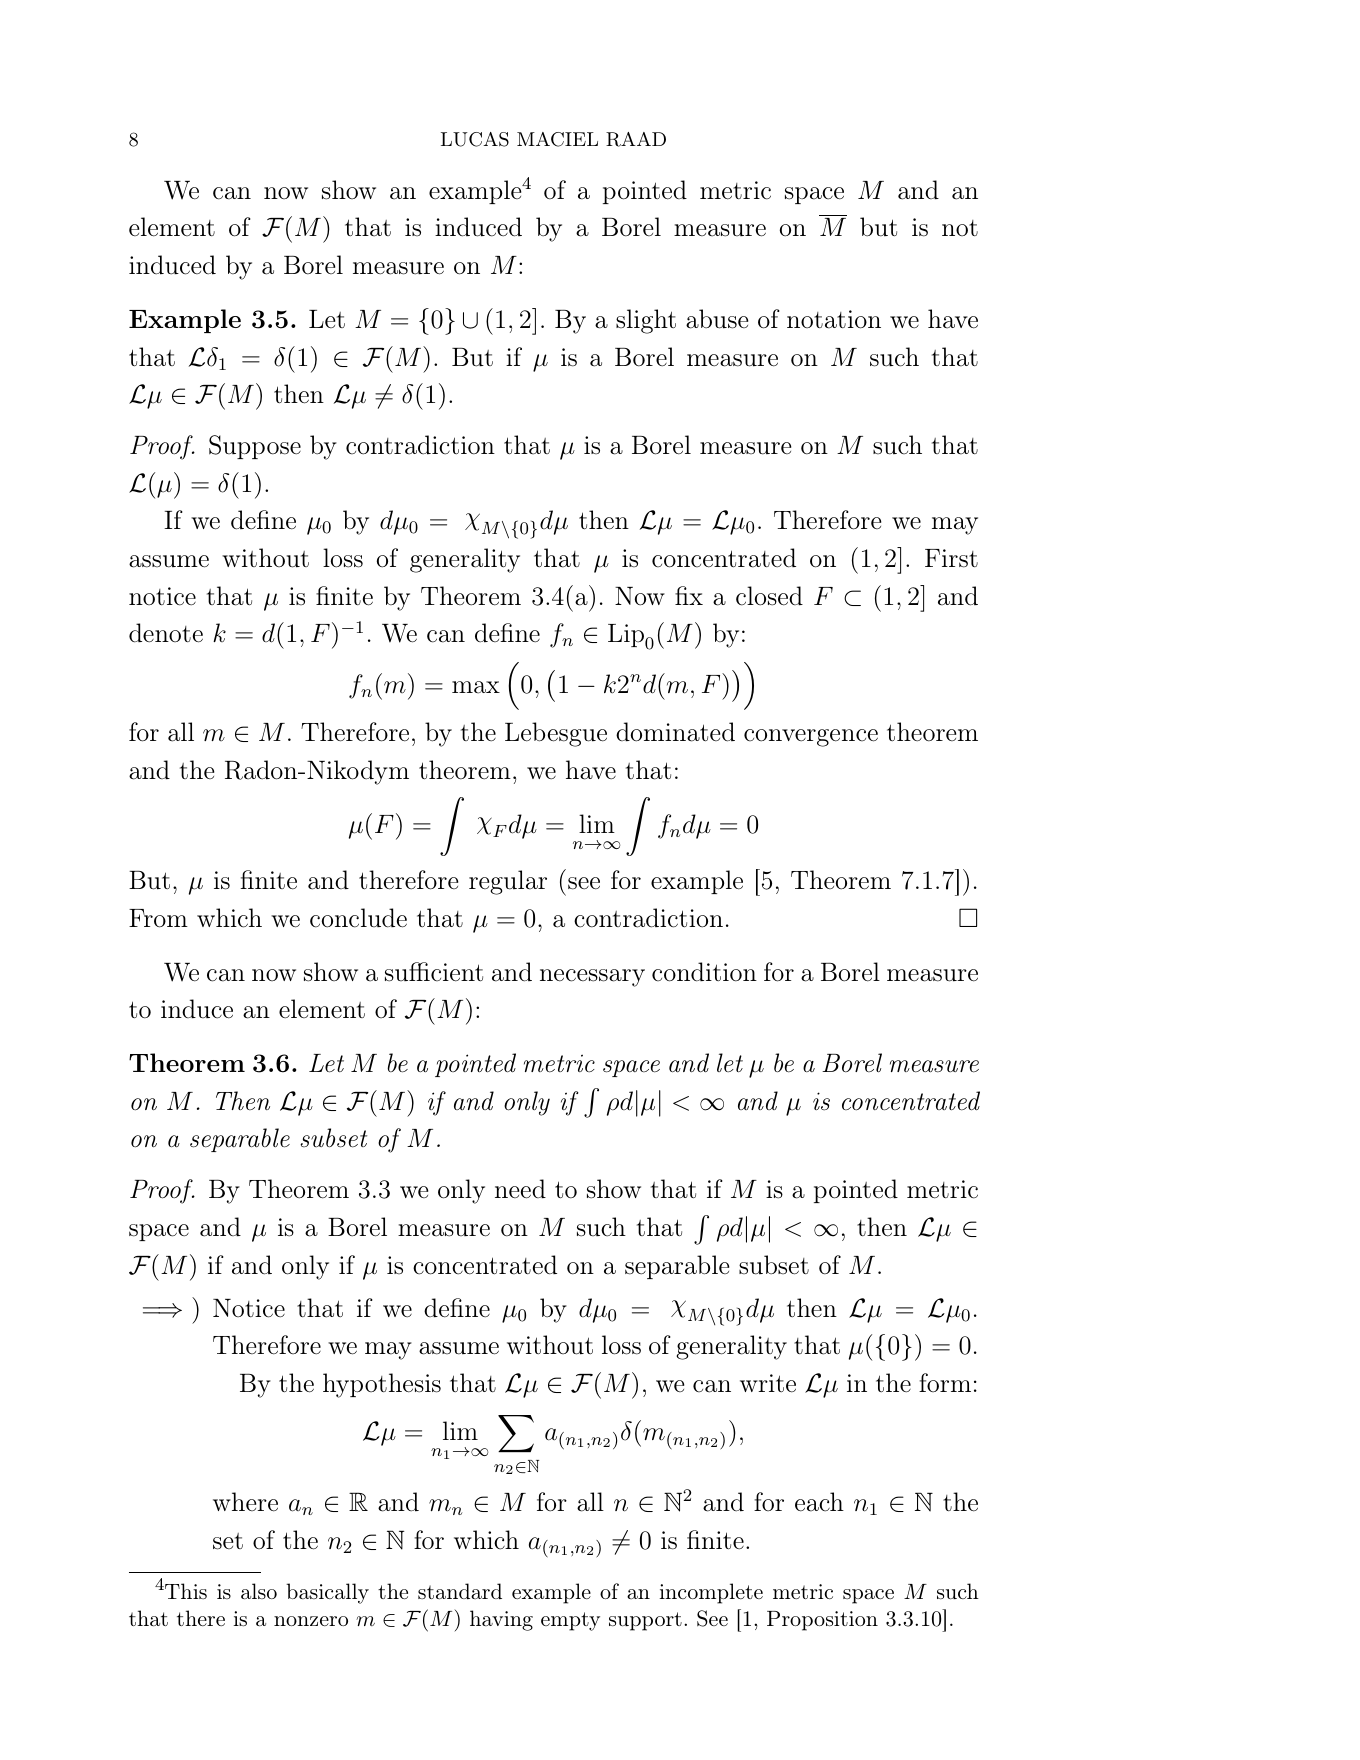
\includegraphics[width=0.82\linewidth]{figures/supporting_answer_page-08.png}
\end{center}

\section*{Identification}

The completion of \((\TP(M),\|\cdot\|_{\TC})\) is the Lipschitz-free space
\(\F(M)\). A finite signed Borel measure \(\sigma\) of total mass zero and
finite first moment determines an element of \(\Lip_0(M)^*\) by
\[
f\mapsto \int_M f\,d\sigma .
\]
Thus \(\sigma\) is approximable by finitely supported transportation problems
in the free-space norm exactly when this functional belongs to \(\F(M)\).

For the positive KR-norm statement, suppose every finite Borel measure on
\(M\) is concentrated on a separable subset. Given positive finite measures
\(\mu,\nu\) with equal mass and finite first moment, concentrate both on a
closed separable subspace \(S\subset M\). Passing to the completion
\(\widehat S\), the measures become measures on a Polish metric space. The
source Theorem 1.13 gives finite-support approximants in the
Kantorovich--Rubinstein norm on \(\widehat S\). Any finitely many atoms lying
in \(\widehat S\setminus S\) can be moved to nearby points of \(S\), changing
the transport cost by an arbitrarily small amount. Therefore \(\TP(M)\) is
dense in \((\M,\|\cdot\|_{\KR})\).

For the negative statement, Raad's Corollary 3.7 gives, whenever the weight of
\(M\) carries a nontrivial measure, a Borel measure \(\mu\) with finite first
moment such that \(L_\mu\notin \F(M)\). Since functions in \(\Lip_0(M)\) vanish
at the base point, \(L_\mu=L_{\mu-\mu(M)\delta_0}\). This signed measure has
total mass zero and finite first moment, hence is a KR measure element. If it
were a KR-norm limit of elements of \(\TP(M)\), then it would also be a limit
in the weaker Lipschitz-dual norm, forcing \(L_\mu\in\F(M)\), a contradiction.

\section*{Dichotomy}

Let \(\kappa_{\mathrm{rvm}}\) be the least real-valued measurable cardinal, if
it exists. Combining the source theorem with Raad's results gives:
\[
\text{\(\TP(M)\) is dense for all finite-first-moment Borel measures on \(M\)}
\]
whenever \(w(M)<\kappa_{\mathrm{rvm}}\), and in particular for every metric
space \(M\) if no real-valued measurable cardinal exists. Conversely, if a
real-valued measurable cardinal exists, then the unrestricted density statement
fails for metric spaces of weight at least \(\kappa_{\mathrm{rvm}}\).

Thus the source's general-metric question has a sharp set-theoretic answer:
below the real-valued-measurable threshold the analogue is true, while above it
there are non-tight Borel measures giving counterexamples.

\section*{Scope Notes}

The supporting paper does not explicitly claim to answer Remark 1.14 of
arXiv:1902.10334; this packet records the reformulation. The earlier packet
on tight-measure TC/KR density is preserved in
\texttt{history/1902.10334\_tight\_measure\_tc\_kr\_density\_partial\_2026\_06\_16/}
as the elementary subcase.

\begin{thebibliography}{9}
\bibitem{OO2019}
S. Ostrovska and M. I. Ostrovskii,
\emph{Generalized transportation cost spaces}, arXiv:1902.10334, 2019.

\bibitem{Raad2024}
L. M. Raad,
\emph{A Characterization of Borel Measures which Induce Lipschitz-Free Space
Elements}, arXiv:2412.13319, version 4, 2025.
\end{thebibliography}

\end{document}
